\documentclass[openany]{book}

\usepackage[margin=1in]{geometry}
\usepackage{amsmath,amsfonts,amsthm, amssymb}
\usepackage{yhmath}
\usepackage{mathrsfs}
\usepackage{mathtools}
\usepackage{xcolor}
\usepackage{graphicx}
\usepackage{comment}
\usepackage{tikz-cd}
\usepackage{quiver}
\renewcommand{\familydefault}{ppl}
\newcommand{\tr}{\text{tr}}
\newcommand{\R}{\mathbb{R}}
\newcommand{\E}{\mathbb{E}}
\newcommand{\Z}{\mathbb{Z}}
\newcommand{\C}{\mathbb{C}}
\newcommand{\F}{\mathbb{F}}
\newcommand{\la}{\langle}
\newcommand{\ra}{\rangle}
\newcommand{\colim}{\text{colim}}
\DeclareMathOperator{\im}{im}
\let\oldemptyset\emptyset
\let\emptyset\varnothing
\newcommand{\tor}{\text{Tor}}
\newcommand{\id}{\text{id}}
\newcommand{\ext}{\text{Ext}}
\newcommand{\ptop}{\text{PTop}}
\newcommand{\pt}{\text{pt}}
\newcommand{\ach}{\text{Ach}}
\newcommand{\Q}{\mathbb{Q}}
\newcommand{\gal}{\text{Gal}}
\newcommand{\diverg}{\operatorname{div}}
\newcommand{\curl}{\operatorname{curl}}

\usepackage{thmtools,thm-restate}

% Fixing mdframed skip below
% See https://tex.stackexchange.com/a/292090/143086
\usepackage[framemethod=TikZ]{mdframed}
\usepackage{xpatch}
\makeatletter
\xpatchcmd{\endmdframed}
	{\aftergroup\endmdf@trivlist\color@endgroup}
	{\endmdf@trivlist\color@endgroup\@doendpe}
	{}{}
\makeatother

\definecolor{huilightpink}{HTML}{fff2fe}
\definecolor{huidarkpink}{HTML}{d955b7}
\declaretheoremstyle[
	mdframed={
		backgroundcolor=huilightpink,
		linecolor=huidarkpink,
		rightline=false,
		topline=false,
		bottomline=false,
		linewidth=2pt,
		innertopmargin=5pt,
		innerbottommargin=8pt,
		innerleftmargin=8pt,
		leftmargin=-2pt,
		skipbelow=2pt,
		nobreak
	},
	headfont=\normalfont\bfseries\color{huidarkpink}
]{huipinkbox}
\declaretheorem[style=huipinkbox,name=Theorem,within=chapter]{thm}
\declaretheorem[style=huipinkbox,name=Theorem,sibling=thm]{theorem}




\begin{comment}
\definecolor{huilightyellow}{HTML}{fff5d6}
\definecolor{huidarkyellow}{HTML}{fcad03}
\declaretheoremstyle[
	mdframed={
		backgroundcolor=huilightyellow,
		linecolor=huidarkyellow,
		rightline=false,
		topline=false,
		bottomline=false,
		linewidth=2pt,
		innertopmargin=5pt,
		innerbottommargin=8pt,
		innerleftmargin=8pt,
		leftmargin=-2pt,
		skipbelow=2pt,
		nobreak
	},
	headfont=\normalfont\bfseries\color{huidarkyellow}
]{huiyellowbox}
\declaretheorem[style=huiyellowbox,name=Proposition,within=chapter]{prop}
\end{comment}



\definecolor{huilightpurple}{HTML}{faf2ff}
\definecolor{huidarkpurple}{HTML}{912ed9}
\declaretheoremstyle[
	mdframed={
		backgroundcolor=huilightpurple,
		linecolor=huidarkpurple,
		rightline=false,
		topline=false,
		bottomline=false,
		linewidth=2pt,
		innertopmargin=5pt,
		innerbottommargin=8pt,
		innerleftmargin=8pt,
		leftmargin=-2pt,
		skipbelow=2pt,
		nobreak
	},
	headfont=\normalfont\bfseries\color{huidarkpurple}
]{huipurplebox}
\declaretheorem[style=huipurplebox,name=Proposition,within=chapter]{prop}



% \definecolor{huilightpurple}{HTML}{faf2ff}
% \definecolor{huidarkpurple}{HTML}{912ed9}
% \declaretheoremstyle[
% 	mdframed={
% 		backgroundcolor=huilightpurple,
% 		linecolor=huidarkpurple,
% 		rightline=false,
% 		topline=false,
% 		bottomline=false,
% 		linewidth=2pt,
% 		innertopmargin=5pt,
% 		innerbottommargin=8pt,
% 		innerleftmargin=8pt,
% 		leftmargin=-2pt,
% 		skipbelow=2pt,
% 		nobreak
% 	},
% 	headfont=\normalfont\bfseries\color{huidarkpurple}
% ]{huipurplebox}
\declaretheorem[style=huipurplebox,name=Lemma,within=chapter]{lem}


\definecolor{lightpink}{HTML}{f0f6fc}
\definecolor{darkpink}{HTML}{2c72b8}
\declaretheoremstyle[
	mdframed={
		backgroundcolor=lightpink,
		linecolor=darkpink,
		rightline=false,
		topline=false,
		bottomline=false,
		linewidth=2pt,
		innertopmargin=5pt,
		innerbottommargin=8pt,
		innerleftmargin=8pt,
		leftmargin=-2pt,
		skipbelow=2pt,
		nobreak
	},
	headfont=\normalfont\bfseries\color{darkpink}
]{pinkbox}
\declaretheorem[style=pinkbox,name=Definition,within=chapter]{defn}


\definecolor{huilightblue}{HTML}{edf9ff}
\definecolor{huidarkblue}{HTML}{4b79db}
\declaretheoremstyle[
	mdframed={
		backgroundcolor=huilightblue,
		linecolor=huidarkblue,
		rightline=false,
		topline=false,
		bottomline=false,
		linewidth=2pt,
		innertopmargin=5pt,
		innerbottommargin=8pt,
		innerleftmargin=8pt,
		leftmargin=-2pt,
		skipbelow=2pt,
		nobreak
	},
	headfont=\normalfont\bfseries\color{huidarkblue}
]{huiblueblox}
\declaretheorem[style=huiblueblox,name=Example,within=chapter]{example}



% \definecolor{huilightblue}{HTML}{edf9ff}
% \definecolor{huidarkblue}{HTML}{4b79db}
% \declaretheoremstyle[
% 	mdframed={
% 		backgroundcolor=huilightblue,
% 		linecolor=huidarkblue,
% 		rightline=false,
% 		topline=false,
% 		bottomline=false,
% 		linewidth=2pt,
% 		innertopmargin=5pt,
% 		innerbottommargin=8pt,
% 		innerleftmargin=8pt,
% 		leftmargin=-2pt,
% 		skipbelow=2pt,
% 		nobreak
% 	},
% 	headfont=\normalfont\bfseries\color{huidarkblue}
% ]{huiblueblox}
% \declaretheorem[style=huiblueblox,name=Example,within=chapter]{example}

% \declaretheoremstyle[
% 	mdframed={
% 		backgroundcolor=huilightblue,
% 		linecolor=huidarkblue,
% 		rightline=false,
% 		topline=false,
% 		bottomline=false,
% 		linewidth=2pt,
% 		innertopmargin=5pt,
% 		innerbottommargin=8pt,
% 		innerleftmargin=8pt,
% 		leftmargin=-2pt,
% 		skipbelow=2pt,
% 		nobreak
% 	},
% 	headfont=\normalfont\bfseries\color{huidarkblue}
% ]{huiblueblox}
\declaretheorem[style=huiblueblox,name=Problem,within=chapter]{prob}



% \declaretheoremstyle[
% 	mdframed={
% 		backgroundcolor=huilightblue,
% 		linecolor=huidarkblue,
% 		rightline=false,
% 		topline=false,
% 		bottomline=false,
% 		linewidth=2pt,
% 		innertopmargin=5pt,
% 		innerbottommargin=8pt,
% 		innerleftmargin=8pt,
% 		leftmargin=-2pt,
% 		skipbelow=2pt,
% 		nobreak
% 	},
% 	headfont=\normalfont\bfseries\color{huidarkblue}
% ]{huiblueblox}
\declaretheorem[style=huiblueblox,name=Exercise,within=chapter]{exer}
\declaretheorem[style=huipinkbox, name=Corollary, within=chapter]{cor}





















\newcommand{\nirwarnsymbol}{%
	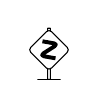
\begin{tikzpicture}[baseline=(x.base)]
		\draw[rounded corners=.01em] (-.05em,-1.07em)rectangle(.05em,.78em);
		\draw[fill=white,rounded corners=1.3] (0,.75em)--(.75em,0)--(0,-.75em)--(-.75em,0)--cycle;
		\draw[line width=0.2mm, line cap=round](-.4em,-1.07em)--(.4em,-1.07em);
		\node(x) at (0,0em) {};
		% Thank you https://tex.stackexchange.com/a/262510
		\draw[
			line cap=but,
			line join=round,
			x=.5em,
			line width=0.5mm,
			y=1*(height("Z")-\pgflinewidth)*(1-sin(10)),
			rotate=-10,
			rounded corners=1.5pt,
		](-0.57, 0.57) -- (0.57, 0.57) -- (-0.57, -0.57) -- (0.57, -0.57);
	\end{tikzpicture}%
}

%%%%%%%%%%%%%%%%%%%%%%%%%%%%%%%%%%%%%%%%%%%% MARGINS
\usepackage{marginnote}
% Thank you https://tex.stackexchange.com/a/472882
% Makes marginnotes always appear on the left, apparently
%
\makeatletter
\long\def\@mn@@@marginnote[#1]#2[#3]{%
	\begingroup
		\ifmmode\mn@strut\let\@tempa\mn@vadjust\else
			\if@inlabel\leavevmode\fi
			\ifhmode\mn@strut\let\@tempa\mn@vadjust\else\let\@tempa\mn@vlap\fi
		\fi
		\@tempa{%
			\vbox to\z@{%
				\vss
				\@mn@margintest
				\if@reversemargin\if@tempswa
						\@tempswafalse
					\else
						\@tempswatrue
				\fi\fi

					\llap{%
						\vbox to\z@{\kern\marginnotevadjust\kern #3
							\vbox to\z@{%
								\hsize\marginparwidth
								\linewidth\hsize
								\kern-\parskip
								%\mn@parboxrestore
								\marginfont\raggedleftmarginnote\strut\hspace{\z@}%
								\ignorespaces#1\endgraf
								\vss
							}%
							\vss
						}%
						\if@mn@verbose
							\PackageInfo{marginnote}{xpos seems to be \@mn@currxpos}%
						\fi
						\begingroup
							\ifx\@mn@currxpos\relax\else\ifx\@mn@currpos\@empty\else
									\kern\@mn@currxpos
							\fi\fi
							\ifx\@mn@currpage\relax
								\let\@mn@currpage\@ne
							\fi
							\if@twoside\ifodd\@mn@currpage\relax
									\kern-\oddsidemargin
								\else
									\kern-\evensidemargin
								\fi
							\else
								\kern-\oddsidemargin
							\fi
							\kern-1in
						\endgroup
						\kern\marginparsep
					}%
			}%
		}%
	\endgroup
}
\makeatother
%
% Mostly for todonotes
\renewcommand{\marginpar}{\marginnote}
%%%%%%%%%%%%%%%%%%%%%%%%%%%%%%%%%%%%%%%%%%%% /MARGINS

\definecolor{nirlightred}{RGB}{250, 220, 220}
\definecolor{nirdarkred}{HTML}{f40000}
\declaretheoremstyle[
	mdframed={
		backgroundcolor=nirlightred,
		linecolor=nirdarkred,
		rightline=false,
		topline=false,
		bottomline=false,
		linewidth=2pt,
		innertopmargin=5pt,
		innerbottommargin=8pt,
		innerleftmargin=8pt,
		leftmargin=-2pt,
		skipbelow=2pt,
		nobreak
	},
	headfont=\normalfont\bfseries\color{nirdarkred}
]{nirredbox}

% \makeatletter
% \declaretheorem[
% 	style=nirredbox,
% 	name=Warning,
% 	sibling=thm,
% 	% without \leavevmode, the first item in a list gets misformatted
% 	postheadhook={\leavevmode\marginnote{\nirwarnsymbol}[-3pt]%
% 	\ifthmt@thisistheone% restatable makes alignment weird
% 		\hspace{-2.2pt}%
% 	\fi}
% ]{warn}
% \makeatother

\newcommand{\nirideasymbol}{%
	
\begin{tikzpicture}[baseline=(x.base)]
		\draw[rounded corners=.01em] (-.05em,-1.07em)rectangle(.05em,.78em);
		\draw[fill=white,rounded corners=1.3] (0,.75em)--(.75em,0)--(0,-.75em)--(-.75em,0)--cycle;
		\draw[line width=0.2mm, line cap=round](-.4em,-1.07em)--(.4em,-1.07em);
		\node(x) at (0,0em) {};
		\node at (0,0em) {{\textbf{!}}};
	\end{tikzpicture}%
}
\renewcommand{\nirwarnsymbol}{%
	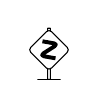
\begin{tikzpicture}[baseline=(x.base)]
		\draw[rounded corners=.01em] (-.05em,-1.07em)rectangle(.05em,.78em);
		\draw[fill=white,rounded corners=1.3] (0,.75em)--(.75em,0)--(0,-.75em)--(-.75em,0)--cycle;
		\draw[line width=0.2mm, line cap=round](-.4em,-1.07em)--(.4em,-1.07em);
		\node(x) at (0,0em) {};
		% Thank you https://tex.stackexchange.com/a/262510
		\draw[
			line cap=but,
			line join=round,
			x=.5em,
			line width=0.5mm,
			y=1*(height("Z")-\pgflinewidth)*(1-sin(10)),
			rotate=-10,
			rounded corners=1.5pt,
		](-0.57, 0.57) -- (0.57, 0.57) -- (-0.57, -0.57) -- (0.57, -0.57);
	\end{tikzpicture}%
}
\makeatletter
\declaretheorem[
	style=nirredbox,
	name=Idea,
	sibling=thm,
	% without \leavevmode, the first item in a list gets misformatted
	postheadhook={\leavevmode\marginnote{\nirideasymbol}[-3pt]%
	\ifthmt@thisistheone% restatable makes alignment weird
		\hspace{-2.2pt}%
	\fi}
]{idea}

\declaretheorem[
	style=nirredbox,
	name=Warning,
	sibling=thm,
	% without \leavevmode, the first item in a list gets misformatted
	postheadhook={\leavevmode\marginnote{\nirwarnsymbol}[-3pt]%
	\ifthmt@thisistheone% restatable makes alignment weird
		\hspace{-2.2pt}%
	\fi}
]{warn}
\makeatother

\title{Calc III Sections
\\ 
\vspace{0.4cm}
\large Fall 2025}






\date{\today}
\author{Hui Sun}


\begin{document}

\maketitle

% \tableofcontents
\newpage


\begin{center}
    \Large Calc III-Week 10 (10/27-31)
\end{center}

\renewcommand\thesection{\arabic{section}}

\noindent
Topics: (1) Divergence and Curl, (2) Double integrals.



% \begin{defn}[flow line]
%     Let ${F}$ be a vector field, a flow line of $F$ is a path $c(t)$ satisfying 
%     \begin{equation*}
%         c'(t)=F(c(t))
%     \end{equation*}
%     (Tangent vector of the path coincides with the given vector field ${F}$).
% \end{defn}

\begin{defn}[divergence]
    Let ${F}$ be a vector field in $\R^3$ $F=(F_1,F_2,F_3)$, the divergence of ${F}$ is the \textbf{scalar field} (assigns one number to an given point $(x, y, z)$), 
    \begin{equation*}
        \diverg F\coloneq\nabla\cdot F=\frac{\partial F_1}{\partial x}+\frac{\partial F_2}{\partial y}+\frac{\partial F_3}{\partial z}
    \end{equation*}
    More generally, if $F=(F_1,\dots, F_n)$ is a vector field on $\R^n$, its divergence is 
    \begin{equation*}
        \diverg F=\sum_{i=1}^n\frac{\partial F_i}{\partial x_i}=\frac{\partial F_1}{\partial x_1}+\dots+\frac{\partial F_n}{\partial x_n}
    \end{equation*}
\end{defn}

\begin{remark}
    We write the divergence as $\nabla\cdot F$ because 
    \begin{equation*}
        \nabla=\left(\frac{\partial}{\partial x_1}, \dots, \frac{\partial}{\partial x_n}\right)
    \end{equation*}
    and if $F=(F_1,\dots, F_n)$, 
    \begin{equation*}
        \diverg F=\frac{\partial F_1}{\partial x_1}+\dots+\frac{\partial F_n}{\partial x_n}=\left(\frac{\partial}{\partial x_1}, \dots, \frac{\partial}{\partial x_n}\right)\cdot(F_1,\dots, F_n)=\nabla\cdot F
    \end{equation*}
\end{remark}


\begin{defn}[curl]
    Let $F$ be a vector field in $\R^3$, writing $F=(F_1,F_2,F_3)$, the \textbf{curl} of $F$ is the vector field 
    \begin{equation*}
        \curl F\coloneq\nabla\times F=\det\begin{bmatrix}
            i&j&k\\
            \frac{\partial}{\partial x}&\frac{\partial}{\partial y}&\frac{\partial}{\partial z}\\
            F_1&F_2&F_3
        \end{bmatrix}
    \end{equation*}
    If $\curl F=0$, then we say the vector field is \textbf{irrotational}.
\end{defn}
% \begin{warn}
%     Irrotational does not mean the vector field doesn't look like rotations.
% \end{warn}

\begin{prop}[gradient is irrotational]
    Let $f\in C^2$, where $f:\R^3\to\R$, viewing $\nabla f$ as a vector field, then
    \begin{equation*}
        \nabla\times(\nabla f)=0
    \end{equation*}    
\end{prop}

\begin{prop}[divergence of a curl vanishes]
    For any $C^2$ vector field $F$, 
    \begin{equation*}
        \nabla\cdot(\nabla\times F)=0
    \end{equation*}
\end{prop}


\begin{prop}[Fubini's Theorem]
    Let $f$ e a continuous function on a rectangular domain $R=[a,b]\times[c,d]$, then 
    \begin{equation*}
        \int_a^b\int_c^df(x,y)dydx=\int_c^d\int_a^bf(x,y)dxdy
    \end{equation*}
\end{prop}


\begin{prob}
    Show that the vector field $V(x,y,z)=(x^2, -y, z)$ is not the curl of any vector field $F$. In other words, there is no vector field $F$ such that 
    \begin{equation*}
        V=\curl F
    \end{equation*}
\end{prob}
% \begin{proof}
%     By the above proposition, if there exists $F$ such that 
%     \begin{equation*}
%         V=\curl F
%     \end{equation*}
%     then 
%     \begin{equation*}
%         \nabla\cdot V=0
%     \end{equation*}
%     However, 
%     \begin{equation*}
%         \nabla\cdot V(x,y,z)=2x\neq 0 \text{ if } x\neq 0
%     \end{equation*}
%     this is a contradiction, hence no such $F$ exists.
% \end{proof}




\begin{prob}[Marsden-Tromba, IV.4, 21]
    Let $F(x,y,z)=(x^2, x^2y, z+zx)$. Can there exist a function $f:\R^3\to\R$ such that $F=\nabla f$?
\end{prob}





\begin{prob}
    Change the order of integration to $dydx$ for the following function:
    \begin{equation*}
        \int_0^1\int_{e^y}^{e}\frac{x}{\ln x}dxdy
    \end{equation*}
\end{prob}
% \begin{proof}
%     It should be 
%     \begin{equation*}
%         \int_1^e\int_{0}^{\ln x}\frac{x}{\ln x}dydx
%     \end{equation*}
% \end{proof}


\begin{prob}
    Change the order of integrations for the following functions:
    \begin{enumerate}
        \item \begin{equation*}
            \int_0^1\int_x^1f(x,y)dydx
        \end{equation*}
        \item \begin{equation*}
            \int_0^1\int_{-y}^{y^3}f(x,y)dxdy
        \end{equation*}
        \item \begin{equation*}
            \int_0^3\int_{2x}^6f(x,y)dydx
        \end{equation*}
        \item \begin{equation*}
            \int_0^1\int_{-\sqrt{y}}^{y^2}f(x,y)dxdy
        \end{equation*}
        \item \begin{equation*}
            \int_0^8\int_{\sqrt[3]{y}}^2f(x,y)dxdy
        \end{equation*}
        \item \begin{equation*}
            \int_0^1\int_{\ln y}^1f(x,y)dxdy
        \end{equation*}
    \end{enumerate}
\end{prob}
% \begin{proof}
%     \begin{enumerate}
%         \item It should be 
%         \begin{equation*}
%             \int_0^1\int_0^yf(x,y)dxdy
%         \end{equation*}
%         \item It should be 
%         \begin{equation*}
%             \int_{-1}^0\int_{-x}^{1}f(x,y)dydx+\int_{0}^1\int_{\sqrt{x}}^1f(x,y)dydx
%         \end{equation*}
%         \item It should be 
%         \begin{equation*}
%             \int_0^6\int_0^{\frac{y}{2}}f(x,y)dxdy
%         \end{equation*}
%         \item It should be \begin{equation*}
%             \int_0^1\int_{\sqrt{x}}^1f(x,y)dydx+\int_{-1}^0\int_{x^2}^1f(x,y)dydx
%         \end{equation*}
%         \item It should be 
%         \begin{equation*}
%             \int_0^2\int_0^{x^3}f(x,y)dydx
%         \end{equation*}
%         \item It should be 
%         \begin{equation*}
%             \int_{-\infty}^0\int_0^{e^x}f(x,y)dydx+\int_0^1\int_0^1f(x,y)dydx
%         \end{equation*}
%     \end{enumerate}
% \end{proof}




























\end{document}